% Auto-generated from 李锡泽_7.12.docx by tools/convert_docx.ps1.
\documentclass[UTF8,11pt,a4paper]{ctexart}
\usepackage[margin=2.54cm]{geometry}
\usepackage{amsmath,amssymb,mathtools}
\usepackage{graphicx}
\graphicspath{{./}{src/}}
\usepackage{subcaption}
\usepackage{booktabs}
\usepackage{float}
\usepackage{cite}
\usepackage{algorithm}
\usepackage{algpseudocode}
\usepackage{tikz}
\usetikzlibrary{arrows.meta,calc,fit,positioning,shapes.geometric,shapes.symbols}
\floatname{algorithm}{算法}
\makeatletter
\renewenvironment{thebibliography}[1]
  {\section{参考文献（References）}%
   \list{\@biblabel{\@arabic\c@enumiv}}%
        {\settowidth\labelwidth{\@biblabel{#1}}%
         \leftmargin\labelwidth
         \advance\leftmargin\labelsep
         \@openbib@code
         \usecounter{enumiv}%
         \let\p@enumiv\@empty
         \renewcommand\theenumiv{\@arabic\c@enumiv}}%
   \sloppy\clubpenalty4000\@clubpenalty\clubpenalty
   \widowpenalty4000%
   \sfcode`\.=\@m}
  {\def\@noitemerr{\@latex@warning{Empty `thebibliography' environment}}%
   \endlist}
\makeatother
\setlength{\parindent}{2em}
\setlength{\parskip}{0.35em}
\begin{document}
\title{面向长期外部性的无人机辅助任务卸载动态激励机制}
\author{李锡泽}
\date{}
\maketitle
\begin{abstract}
在无人机（UAV）辅助边缘计算网络中，无人机可作为空中移动边缘服务器，为地面用户提供灵活的计算卸载服务。然而，多个用户对有限机载计算资源的竞争容易造成资源拥塞，进而增加任务时延并降低资源利用效率。为缓解资源竞争带来的拥塞并提升资源配置效率，有必要设计合理的定价激励机制，协调无人机与用户之间的资源交易。本文将无人机与地面用户之间的动态资源交易过程建模为部分可观测随机博弈（POSG）。在该博弈中，无人机作为计算资源提供方，联合决策任务接收与服务位置，以最大化长期折扣社会福利；地面用户根据自身私有的时延敏感类型选择报告策略，以最大化长期折扣效用。针对策略性报告导致的资源错配问题，本文提出由无人机执行的面向长期外部性的动态激励机制。该机制针对每个用户构造移除该用户的反事实环境，利用无人机 SAC 学习得到的动作价值函数，比较反事实环境下重新优化决策与沿用完整系统决策时其余参与者的长期折扣社会福利，并以二者差值确定外部性支付。无人机和各用户分别采用独立的离散动作 SAC，前者学习任务接收与服务位置策略，后者学习类型报告策略。仿真结果表明，与即时 VCG 定价和无定价基线相比，所提机制能够获得更高且更稳定的系统收益，并有效降低用户的类型报告偏差，说明该机制能够在提升长期资源配置效率的同时抑制策略性虚报。

\noindent\textbf{关键词：}无人机辅助移动边缘计算；动态激励机制；多智能体强化学习
\end{abstract}
\section{引言（Introduction）}
现有移动设备受限于物理体积和本地算力，难以满足 5G 场景日益增长的计算需求。移动边缘计算（Mobile Edge Computing, MEC）通过将任务卸载至邻近边缘服务器，为资源受限设备提供计算支撑。在 UAV 辅助 MEC 网络中，UAV 可作为空中移动边缘服务器，为基站覆盖不足区域的用户提供卸载服务。已有研究围绕 UAV 部署与任务卸载、UAV 高度、用户关联及卸载决策等问题展开\cite{shen2023joint,hui2024optimal,wang2024distributed}。然而，MEC 中任务到达、信道状态和资源约束具有动态性，卸载、资源分配与 UAV 位置控制相互耦合，静态优化难以获得长期有效策略。强化学习（Reinforcement Learning, RL）通过环境交互学习决策策略，适用于此类动态序贯问题，并已用于 MEC 中的任务调度、卸载和轨迹优化\cite{tian2023deep,ju2024multi}。现有研究多以时延、能耗和吞吐量为目标，较少考虑用户私有信息与参与激励。鉴于 UAV 承担飞行、通信和计算成本、用户追求自身效用最大化，有必要设计兼顾动态决策与信息激励的机制，促进双方持续参与计算卸载。

在 MEC 场景中，拍卖机制可通过联合设计供需匹配、资源分配与支付规则，协调私有信息条件下的计算和通信资源交易，通常以社会福利作为重要优化目标。双边拍卖分别接收任务请求方的报价与服务提供方的要价，通过匹配确定交易对象和资源分配；组合拍卖则允许参与者针对任务及其所需资源组合提交偏好，以处理资源需求的耦合性。相关研究已探索多轮资源交易和真实组合拍卖。例如，Xiao 等研究面向边缘计算的多轮拍卖资源分配，以社会福利最大化为目标协调多用户与多服务器之间的供需关系\cite{xiao2023multiround}；Su 等面向工业物联网移动边缘计算提出真实组合拍卖机制，在组合资源配置中兼顾真实性与社会福利最大化\cite{su2022truthful}。这些工作为私有信息条件下的边缘资源配置与卸载激励研究提供了参考。

然而，将上述拍卖机制按单轮交易独立执行，难以反映 MEC 系统的状态演化及其长期影响。在 UAV 辅助 MEC 中，服务位置、通信状态和资源配置均随时间变化，参与者的当前决策还会影响后续服务过程及其他参与者收益。因此，仅依据即时状态确定交易结果和支付，难以准确评估参与者在长期过程中的外部性。VCG 拍卖以参与者对其他参与者造成的外部性为支付依据，兼顾资源配置效率与真实报告激励。Wu 等进一步将其用于连续参与的联邦学习场景，提出长期自适应 VCG 拍卖机制\cite{wu2024longterm}。对于动态 UAV 辅助 MEC，定价机制需要同时处理动态服务决策与参与者私有信息，并在支付中反映当前参与对未来状态演化和社会福利的累计影响。因此，该场景需要面向持续交互过程的长期外部性定价，使支付能够体现参与者对其他参与者的跨期影响。

针对上述问题，本文借鉴动态枢轴机制的思想\cite{bergemann2010dynamic}，构建面向跨期外部性的 UAV 辅助 MEC 动态激励机制。本文不以当前时隙的福利差异作为唯一计价依据，而是构造包含未来状态转移的反事实环境，利用长期 Q 值估计某一用户参与后对其余参与者累计折扣社会福利的影响，并据此确定长期外部性支付，从而在支付计算中纳入 UAV 位置演化和资源配置的跨时隙影响。

本文主要贡献如下：

\begin{itemize}
    \item 面向任务动态到达、UAV 位置随时隙变化且机载资源受限的 UAV 辅助 MEC 场景，构建包含 UAV 服务平台与移动用户的长期动态激励模型，将用户私有时延敏感类型、任务接收、服务位置和支付规则纳入统一的长期社会福利分析框架。
    \item 提出基于反事实长期 Q 值的跨期外部性定价方法。针对每个用户构造移除该用户的反事实环境，比较重新优化动作与完整系统动作删除该用户任务后的长期 Q 值，并以二者差值确定外部性支付，从而将 VCG 定价扩展至状态持续演化的动态卸载过程。
    \item 构建基于多智能体离散动作 SAC 的策略学习与支付计算框架，分别学习 UAV 的任务接收与服务位置策略、移动用户的类型上报策略，并通过随机采样反事实分支降低长期外部性估计中的重复环境交互开销。
\end{itemize}

\section{系统模型（System Model）}
考虑由一架 UAV 和移动用户集合 $N=\{1,2,\ldots,N\}$ 组成的 UAV 辅助 MEC 系统，其中节点 $0$ 表示 UAV，节点 $n\in N$ 表示第 $n$ 个移动用户。系统在离散时隙中运行。在每个时隙内，UAV 基于当前系统状态联合确定目标服务位置和任务接收结果；被接收的任务经上行链路传输后由 UAV 处理，其余任务在本地完成。下文依次建立通信、计算卸载和 UAV 能耗模型。
\subsection{通信模型}
考虑用户 $n$ 在时隙 $t$ 向 UAV 上传卸载任务。UAV 与用户 $n$ 之间的上行链路可能为视距（LoS）或非视距（NLoS）链路，其中 LoS 链路的概率表示为：
\begin{equation}
Pr_{n,LoS}\left(t\right)=\frac{1}{1+\mu _{1}e^{-\mu _{2}\left(\phi _{n}(t)-\mu _{1}\right)}}
\end{equation}
其中，$\mu _{1}$ 和 $\mu _{2}$ 为环境常数，$\phi _{n}\left(t\right)$ 表示 UAV 与用户 $n$ 之间的仰角，其定义为：
\begin{equation}
\phi _{n}(t)=\arcsin\left(\frac{z_{0,n}(t)}{\left(l_{0}\left(t\right)-l_{n}\left(t\right)\right)}\right)
\end{equation}
式中，$z_{0,n}(t)$ 为 UAV 与用户 $n$ 之间的高度差，$l_{0}\left(t\right)$ 和 $l_{n}\left(t\right)$ 分别表示 UAV 和用户 $n$ 的位置。相应地，NLoS 链路的概率由 LoS 概率的补集给出\cite{alhourani2014modeling}：
\begin{equation}
Pr_{n,NLoS}\left(t\right)=1-Pr_{n,LoS}\left(t\right)
\end{equation}
在给定传播状态 $\nu$ 下，UAV 与用户 $n$ 之间的路径损耗建模为
\begin{equation}
\chi _{0,n}\left(t\right)=\eta _{\nu}\left(l_{0}\left(t\right)-l_{n}\left(t\right)\right)_{2}^{-\alpha _{\nu}},\nu \in \{\mathrm{LoS},\mathrm{NLoS}\}
\end{equation}
其中，$\eta _{\nu}$ 为参考路径损耗常数，$\alpha _{\nu}$ 为路径损耗指数。为刻画小尺度衰落，假设信道衰落系数服从 Nakagami-$m$ 分布，即
\begin{equation}
h_{0,n}\left(t\right)\sim \mathrm{Nakagami}\left(m_{\nu}\right), \nu \in \{\mathrm{LoS},\mathrm{NLoS}\}
\end{equation}
由路径损耗和小尺度衰落共同决定的信道增益为
\begin{equation}
g_{0,n}\left(t\right)=\left(h_{0,n}\left(t\right)\right)^{2}\chi _{0,n}\left(t\right)
\end{equation}
据此，用户 $n$ 向 UAV 的上行传输速率 $\rho _{n}\left(t\right)$ 可表示为
\begin{equation}
\rho _{n}\left(t\right)=B \left(1+\frac{P_{n}g_{0,n}\left(t\right)}{\sigma ^{2}}\right)
\end{equation}
其中，$B$ 为信道带宽，$P_{n}$ 为用户 $n$ 的发射功率，$\sigma ^{2}$ 为高斯噪声功率。若用户 $n$ 在时隙 $t$ 向 UAV 卸载的数据量为 $D_{n}\left(t\right)$，则对应的上传时延为
\begin{equation}
\tau _{n}^{trans}\left(t\right)=\frac{D_{n}\left(t\right)}{\rho _{n}\left(t\right)}
\end{equation}
\subsection{计算卸载模型}
用户 $n$ 在时隙 $t$ 产生的数据量为 $D_{n}\left(t\right)$ 的计算任务。设单位比特任务需要 $\xi$ 个 CPU 周期，则该任务的计算量为 $L_{n}\left(t\right)=D_{n}\left(t\right)\xi$。任务可在本地执行，也可卸载至 UAV 处理\cite{you2017energy}。

设 UAV 的总计算能力为 $F_{\mathrm{uav}}$，并采用按任务量比例分配的计算资源分配策略。定义卸载决策变量 $x_{n}\left(t\right)\in \{0,1\}$，其中 $x_{n}\left(t\right)=1$ 表示任务卸载至 UAV，$x_{n}\left(t\right)=0$ 表示任务在本地执行。则 UAV 分配给用户 $n$ 的计算频率为
\begin{equation}
f_{n}^{\mathrm{uav}}\left(t\right)=x_{n}\left(t\right)\frac{D_{n}\left(t\right)\xi }{\sum_{k=1}^{N} x_{k}\left(t\right)D_{k}\left(t\right)\xi }F_{\mathrm{uav}}.
\end{equation}
对于被卸载的任务，UAV 侧的计算时延为
\begin{equation}
\tau _{n}^{off}\left(t\right)=\frac{D_{n}\left(t\right)\xi }{f_{n}^{\mathrm{uav}}\left(t\right)}.
\end{equation}
因此，用户 $n$ 的任务完成时延由卸载路径或本地计算路径决定，表示为
\begin{equation}
\tau _{n}\left(t\right)=x_{n}\left(t\right)\left(\tau _{n}^{off}\left(t\right)+\tau _{n}^{trans}\left(t\right)\right)+\left(1-x_{n}\left(t\right)\right)\tau _{n}^{local}\left(t\right)
\end{equation}
其中，本地计算时延为
\begin{equation}
\tau _{n}^{local}\left(t\right)=\frac{D_{n}\left(t\right)\xi }{f_{n}^{local}}
\end{equation}
式中，$f_{n}^{local}$ 为用户 $n$ 的本地 CPU 计算频率。
\subsection{UAV 能耗模型}
在时隙 $t$ 内，UAV 的能耗由飞行部署、悬停服务和任务计算三部分构成。设 $P^{fly}$ 和 $P^{hov}$ 分别表示 UAV 的飞行功率和悬停功率。

在时隙开始时，UAV 根据轨迹规划结果从上一位置 $l_{0}(t-1)$ 移动至目标位置 $l_{0}(t)$。假设 UAV 以恒定速度 $V_{\mathrm{uav}}$ 飞行，则移动能耗为
\begin{equation}
E_{move}(t)=P^{fly}\cdot \frac{\left(l_{0}(t)-l_{0}(t-1)\right)}{V_{\mathrm{uav}}}
\end{equation}
UAV 抵达目标位置后，为被接收任务提供通信与计算服务，其悬停能耗建模为
\begin{equation}
E_{hov}(t)=\sum_{n=1}^{N} x_{n}(t)P^{hov}[\tau _{n}^{trans}(t)+\tau _{n}^{off}(t)]
\end{equation}
此外，根据 CMOS 动态功耗模型，UAV 的计算能耗与分配的计算频率有关\cite{mao2016dynamic}。设芯片的有效电容系数为 $\kappa_{\mathrm{uav}}$，则 UAV 在时隙 $t$ 处理卸载任务的计算能耗为
\begin{equation}
E_{comp}(t)=\sum_{n=1}^{N} x_{n}(t)\kappa_{\mathrm{uav}} \xi D_{n}(t)(f_{n}^{\mathrm{uav}}(t))^{2}
\end{equation}
因此，UAV 在时隙 $t$ 的总能耗为
\begin{equation}
E_{0}(t)=E_{move}(t)+E_{hov}(t)+E_{comp}(t)
\end{equation}
上述模型共同决定用户任务时延与 UAV 能耗，并将在下一节用于构造参与者效用和系统社会福利。
\section{问题建模（Problem Formulation）}
\subsection{动态激励机制}
为刻画 UAV 辅助 MEC 中任务接收与轨迹控制的时序耦合，本文构建基于类型报告和外部性定价的长期动态激励机制\cite{clarke1971multipart}。由于 UAV 的位置随时隙演化，当前决策会影响后续服务条件与资源分配，因此需要在动态过程中联合确定资源分配与支付规则。

其中，UAV 作为服务平台，负责分配计算资源并确定目标服务位置；移动用户作为机制参与者，通过类型上报参与 UAV 计算资源分配。用户 $n$ 在时隙 $t$ 的私有类型为真实时延敏感度 $\theta _{n}(t)\in [0,1]$，向 UAV 提交的类型报告记为 $\hat{\theta }_{n}(t)$。由于用户以自身效用最大化为目标，其上报值可能偏离真实类型。

在时隙 $t$ 开始时，系统的公共物理状态由 UAV 与各用户在上一时隙的位置，即 $l_{0}(t-1)$ 和 $l_{n}(t-1)$，以及本时隙到达的任务量 $D_{n}(t)$ 共同构成。用户首先提交上报信息；随后，UAV 根据当前状态和全部上报，联合确定任务接收决策 $x_{n}(t)$ 与目标服务位置 $l_{0}(t)$。

动作执行后，系统获得用户 $n$ 在时隙 $t$ 的任务完成时延 $\tau _{n}\left(t\right)$。据此，用户 $n$ 的单步效用定义为准线性形式：
\begin{equation}
U_{n}(t)=-\theta _{n}(t)\tau _{n}\left(t\right)-p_{n}(t)
\end{equation}
其中，$p_{n}(t)$ 为该用户占用计算资源所缴纳的支付费用。进一步地，定义 UAV 在时隙 $t$ 的效用为
\begin{equation}
U_{0}\left(t\right)=\sum_{n=1}^{N} p_{n}\left(t\right)-\beta E_{0}\left(t\right)
\end{equation}
其中，$E_{0}\left(t\right)$ 表示 UAV 在该时隙的总能耗，$\beta$ 为能耗成本系数，用于刻画能量消耗对系统效益的影响。因此，时隙 $t$ 的即时社会福利可定义为所有参与方效用之和，即
\begin{equation}
W(t)=U_{0}(t)+\sum_{n=1}^{N} U_{n}(t)=-\sum_{n=1}^{N} \theta _{n}\left(t\right)\tau _{n}\left(t\right)-\beta E_{0}(t)
\end{equation}
\subsection{长期优化问题}
在动态 UAV 辅助边缘计算场景中，任务到达、用户状态与 UAV 位置均随时间演化，当前决策不仅影响即时资源配置结果，还会改变后续时隙的系统状态。因此，动态激励机制需要同时考虑系统层面的长期资源配置效率与用户层面的个体决策激励，在优化长期社会福利的同时，兼顾用户的类型上报激励与持续参与意愿。基于上述目标，本文分别从 UAV 服务平台和移动用户两个层面构建长期优化问题。

\noindent\textbf{UAV 侧长期社会福利优化：}
作为服务平台，UAV 根据当前系统状态与用户类型报告，在各时隙联合确定任务接收决策和目标服务位置。为刻画当前决策对未来系统演化的影响，UAV 以期望折扣累计社会福利最大化为目标，其优化问题表述为
\begin{equation}
\begin{aligned}
\max_{\{x_n(t)\},\,\{l_0(t)\}} \quad & \mathbb{E}\left[\sum_{t=0}^{T}\gamma^t W(t)\right] \\
\text{s.t.} \quad & x_n(t)\in\{0,1\}, && \forall n\in N,\ \forall t, \\
& l_0(t)\in L, && \forall t.
\end{aligned}
\end{equation}
其中，$\gamma\in[0,1)$ 为折扣因子，$\mathbb{E}[\cdot]$ 表示对任务到达、状态转移及策略随机性等不确定因素取期望；约束条件分别限定任务接收变量的取值范围和 UAV 的可选服务位置。

\noindent\textbf{用户侧长期效用优化：}
移动用户作为具有自利性的机制参与者，其决策目标并非直接最大化系统社会福利，而是在给定机制规则及其他参与者策略的条件下最大化自身效用。对于任意用户 $n$，其决策变量为各时隙提交的类型报告 $\hat{\theta }_{n}(t)$，相应的长期优化问题表述为
\begin{equation}
\begin{aligned}
\max_{\{\hat{\theta}_n(t)\}} \quad & \mathbb{E}\left[\sum_{t=0}^{T}\gamma^t U_n(t)\right] \\
\text{s.t.} \quad & \hat{\theta}_n(t)\in[0,1], && \forall t.
\end{aligned}
\end{equation}
用户效用 $U_n(t)$ 同时取决于任务完成时延和支付，因此，支付规则会直接影响用户的类型报告策略。综上，本文旨在联合设计任务接收、UAV 轨迹控制与支付规则，协调平台侧的长期社会福利目标和用户侧的长期效用目标，从而在兼顾用户上报激励与参与意愿的同时，提高系统的长期资源配置效率。
\section{算法设计（Algorithm Design）}
\subsection{多智能体部分可观测随机博弈建模}
为求解前述长期社会福利优化问题，本文将 UAV 辅助 MEC 系统建模为部分可观测随机博弈（Partially Observable Stochastic Game, POSG）。在该框架下，UAV 根据用户上报学习任务接收与轨迹控制策略，各移动用户则基于局部信息学习上报策略。该博弈记为 $G=\langle I,S,\{Z_i\}_{i\in I},\{A_i\}_{i\in I},P,\{r_i\}_{i\in I},\gamma\rangle$，其中，$I$、$S$、$Z_i$ 和 $A_i$ 分别表示智能体集合、全局状态空间、智能体 $i$ 的局部观测空间和动作空间；$P\bigl(s(t+1)\mid s(t),a(t)\bigr)$ 为状态转移概率，$r_i$ 为即时奖励函数，$\gamma$ 为折扣因子。智能体集合为 $I=\{0\}\cup N$，其中 $0$ 表示 UAV 智能体。为描述环境状态，时隙 $t$ 的全局状态定义为
\begin{equation}
s(t)=\left\{l_0(t-1),\{l_n(t-1)\}_{n=1}^{N},\{D_n(t)\}_{n=1}^{N},\{\theta_n(t)\}_{n=1}^{N}\right\}.
\end{equation}
\subsubsection{UAV 智能体}
UAV 在时隙 $t$ 的局部观测为
\begin{equation}
o_{0}(t)=\left\{l_{0}(t-1),\{l_{n}(t-1)\}_{n=1}^{N},\{D_{n}(t)\}_{n=1}^{N},\{\hat{\theta }_{n}(t)\}_{n=1}^{N}\right\}.
\end{equation}
其动作为任务接收与目标服务位置构成的联合控制动作：
\begin{equation}
a_{0}(t)=\left(\{x_{n}(t)\}_{n=1}^{N},l_{0}(t)\right).
\end{equation}
UAV 的即时奖励取为系统即时社会福利：
\begin{equation}
r_{0}\left(t\right)=W\left(t\right)
\end{equation}
\subsubsection{移动用户智能体}
第 $n$ 个移动用户在时隙 $t$ 的局部观测为
\begin{equation}
o_{n}(t)=\left\{l_{n}(t-1),l_{0}(t-1),D_{n}(t),\theta _{n}(t)\right\}.
\end{equation}
任务量 $D_n(t)$ 和真实时延敏感度 $\theta_n(t)$ 使用户能够根据信息状态调整上报策略。用户的动作为向 UAV 提交的时延敏感度上报：
\begin{equation}
a_{n}(t)=\hat{\theta }_{n}(t).
\end{equation}
其即时奖励定义为单时隙效用：
\begin{equation}
r_{n}(t)=U_{n}(t).
\end{equation}
在每个时隙开始时，环境给定全局状态 $s(t)$。各移动用户基于 $o_n(t)$ 生成类型上报动作 $a_n(t)$，UAV 接收全部上报后依据策略 $\pi_0(a_0(t)\mid o_0(t))$ 生成联合控制动作 $a_0(t)$。随后，环境执行任务卸载、传输与计算，得到用户时延 $\tau_n(t)$ 和相应的长期外部性支付 $p_n(t)$，并依据上述奖励函数反馈各智能体。最后，环境转移至 $s(t+1)$，训练过程利用该转移更新策略。
\subsection{基于 SAC 的策略学习}
UAV 依赖策略 $\pi _{0}(a_{0}(t)\mid o_{0}(t))$ 将局部观测转化为联合控制动作，而各移动用户 $n$ 则通过策略 $\pi _{n}(a_{n}(t)\mid o_{n}(t))$ 生成相应的上报动作。给定 UAV 的局部观测 $o_{0}(t)$ 和联合控制动作 $a_{0}(t)$，在系统联合策略 $\left(\pi _{0},\pi _{n},\forall n\in N\right)$ 下，UAV 的状态--动作值函数（Q 函数）定义为：
\begin{equation}
Q_{0}\left(o_{0}\left(t\right),a_{0}\left(t\right)\right)=\max_{\pi _{0}}\mathbb{E}\left[\sum_{\nu =t}^{T} \gamma ^{\nu -t}r_{0}\left(\nu \right)\mid o_{0}\left(t\right),a_{0}\left(t\right)\right]
\end{equation}
其中，$\mathbb{E}[\cdot]$ 表示对未来所有轮次状态演化和动作选择的期望，$\gamma$ 为折扣因子。最优化该 Q 值的最佳响应策略 $\pi _{0}^{*}$ 表示为：
\begin{equation}
\pi _{0}^{*}=\operatorname*{arg\,max}_{\pi _{0}}Q_{0}\left(o_{0}(t),a_{0}(t)\right)
\end{equation}
同理，给定移动用户 $n$ 的局部观测 $o_{n}\left(t\right)$ 和动作 $a_{n}\left(t\right)$，用户 $n$ 的 Q 函数定义为：
\begin{equation}
Q_{n}\left(o_{n}\left(t\right),a_{n}\left(t\right)\right)=\max_{\pi _{n}}\mathbb{E}\left[\sum_{\nu =t}^{T} \gamma ^{\nu -t}r_{n}\left(\nu \right)\mid o_{n}\left(t\right),a_{n}\left(t\right)\right]
\end{equation}
用户 $n$ 的最佳响应策略 $\pi _{n}^{*}$ 则表示为：
\begin{equation}
\pi _{n}^{*}=\operatorname*{arg\,max}_{\pi _{n}}Q_{n}\left(o_{n}(t),a_{n}(t)\right)
\end{equation}
针对动态环境下联合决策变量连续、系统状态随时间演化且难以获得精确解析解的问题，本文采用 SAC 算法求解长期优化策略\cite{haarnoja2018soft}。
与传统强化学习仅最大化期望累积回报不同，SAC 在目标函数中引入策略熵项，以鼓励策略保持适当随机性，避免过早收敛到局部最优。其最大熵目标函数可表示为
\begin{equation}
\begin{aligned}
J\left(\pi _{m}\right)=E_{a_{m}\sim \pi _{m}}\left(\sum_{\nu =t}^{T} \gamma ^{\nu -t}\left(r_{m}\left(\nu \right)-\alpha  \pi _{m}\left(a_{m}\left(\nu \right)\mid o_{m}\left(\nu \right)\right)\right)\right)
\end{aligned}
\end{equation}
$m\in \left\{0,1,\ldots ,N\right\}$ 代表 UAV 和移动用户智能体。
在最大熵强化学习框架下，第 $m$ 个智能体对应的状态价值函数可表示为
\begin{equation}
\begin{aligned}
V_{m}\left(o_{m}\left(t\right)\right)=E_{a_{m}\left(t\right)\sim \pi _{m}}\left(Q_{m}\left(o_{m}\left(t\right),a_{m}\left(t\right);\hat{\omega }_{m}\right)-\alpha  \pi _{m}\left(a_{m}\left(t\right)\mid o_{m}\left(t\right);\psi _{m}\right)\right)
\end{aligned}
\end{equation}
其中，$\hat{\omega }_{m}$ 表示目标 Q 网络参数，$\psi _{m}$ 表示策略网络参数。由此，第 $m$ 个智能体的时序差分目标可进一步写为
\begin{equation}
\begin{aligned}
y_{m}\left(t\right)=r_{m}\left(t\right)+\gamma V_{m}\left(o_{m}\left(t+1\right)\right)
\end{aligned}
\end{equation}
基于上述时序差分目标，Q 网络损失函数定义为
\begin{equation}
\begin{aligned}
L\left(\omega _{m}\right)=E_{\left(o_{m}\left(t\right),a_{m}\left(t\right),r_{m}\left(t\right),o_{m}\left(t+1\right)\right)\sim D_{m}}\left(\frac{1}{2}\left(Q_{m}\left(o_{m}\left(t\right),a_{m}\left(t\right);\omega _{m}\right)-y_{m}\left(t\right)\right)^{2}\right)
\end{aligned}
\end{equation}
其中，$\omega _{m}$ 表示第 $m$ 个智能体在线 Q 网络的参数，$D_{m}$ 表示其经验回放池。策略网络损失函数可以表示为
\begin{equation}
\begin{aligned}
L\left(\psi _{m}\right)=E_{o_{m}\left(t\right)\sim D_{m}, a_{m}\left(t\right)\sim \pi _{m}}\left(\alpha  \pi _{m}\left(a_{m}\left(t\right)\mid o_{m}\left(t\right);\psi _{m}\right)-Q_{m}\left(o_{m}\left(t\right),a_{m}\left(t\right);\omega _{m}\right)\right)
\end{aligned}
\end{equation}
该损失函数表明，策略网络在更新过程中不仅倾向于选择具有较高动作价值的行为，同时在熵项作用下保持适当的随机性，从而在探索与利用之间取得平衡。
基于上述损失函数，第 $m$ 个智能体的在线 Q 网络参数和目标 Q 网络可通过梯度下降方式更新为
\begin{equation}
\begin{aligned}
\omega _{m}\leftarrow \omega _{m}-\eta _{Q}\nabla _{\omega _{m}}L\left(\omega _{m}\right)
\end{aligned},
\end{equation}
\begin{equation}
\begin{aligned}
\hat{\omega }_{m}\leftarrow \rho \omega _{m}+\left(1-\rho \right)\hat{\omega }_{m},
\end{aligned}
\end{equation}
其中，$\eta _{Q}$ 表示 Q 网络的学习率。目标 Q 网络参数 $\hat{\omega }_{m}$ 采用软更新方式迭代。
类似地，策略网络参数 $\psi _{m}$ 通过最小化策略损失函数进行更新，即
\begin{equation}
\begin{aligned}
\psi _{m}\leftarrow \psi _{m}-\eta _{\pi }\nabla _{\psi _{m}}L\left(\psi _{m}\right)
\end{aligned}
\end{equation}
其中，$\eta _{\pi }$ 表示策略网络的学习率。
为了使策略熵在训练过程中能够自动调节，SAC 通常采用温度参数 $\alpha _{m}$ 的自适应更新机制。设目标熵为 $H_{m}$，则对应的损失函数可写为
\begin{equation}
\begin{aligned}
L\left(\alpha _{m}\right)=E_{o_{m}\left(t\right)\sim D_{m}, a_{m}\left(t\right)\sim \pi _{m}}\left(-\alpha _{m} \pi _{m}\left(a_{m}\left(t\right)\mid o_{m}\left(t\right);\psi _{m}\right)-\alpha _{m}H_{m}\right)
\end{aligned}
\end{equation}
对于温度参数 $\alpha _{m}$，其更新方式为
\begin{equation}
\begin{aligned}
\alpha _{m}\leftarrow \alpha _{m}-\eta _{\alpha }\nabla _{\alpha _{m}}L\left(\alpha _{m}\right),
\end{aligned}
\end{equation}
其中，$\eta _{\alpha }$ 表示温度参数的学习率。
\subsection{基于长期外部性的支付规则}
为刻画用户 $n$ 对其余参与者造成的跨期外部性，本文借鉴动态枢轴机制的外部性定价思想构造长期外部性支付规则\cite{bergemann2010dynamic}。给定 UAV 动作 $a_{0}(t)$，用户 $k$ 在时隙 $t$ 的当期价值定义为
\begin{equation}
v_{k}(a_{0}(t);\theta _{k}(t))=-\theta _{k}(t)\tau _{k}(a_{0}(t)),\qquad k\in N.
\end{equation}
UAV 的当期价值为 $v_{0}(a_{0}(t))=-\beta E_{0}(a_{0}(t))$。记 $\boldsymbol{\theta}^{-n}(t)=\{\theta _{k}(t)\}_{k\in N\setminus \{n\}}$ 为剩余用户的类型向量，则反事实环境中的即时社会福利为
\begin{equation}
W^{-n}(a_{0}(t);\boldsymbol{\theta}^{-n}(t))=v_{0}(a_{0}(t))+\sum_{k\in N\setminus \{n\}}v_{k}(a_{0}(t);\theta _{k}(t)).
\end{equation}
从下一时隙起的期望长期社会福利定义为
\begin{equation}
\mathcal{W}^{-n}(t+1\mid a_{0}(t))=\mathbb{E}\left[\sum_{\nu=t+1}^{T}\gamma^{\nu-(t+1)}W^{-n}(a_{0}(\nu);\boldsymbol{\theta}^{-n}(\nu))\mid a_{0}(t)\right].
\end{equation}
其中，$a_{0}^{*}(t)$ 表示完整系统的最优动作，$a_{0}^{*,-n}(t)$ 表示移除用户 $n$ 后重新求得的最优动作。从 $a_{0}^{*}(t)$ 中删去用户 $n$ 对应的任务接收决策，所得动作记为 $\Pi_{-n}(a_{0}^{*}(t))$。为简洁起见，以下以 $v_{j}(a)$ 表示时隙 $t$ 内参与者 $j$ 在动作 $a$ 下的当期价值。则用户 $n$ 的长期外部性支付为
\begin{equation}
\begin{aligned}
p_{n}(t)={}&\sum_{j\in I\setminus\{n\}}\left[v_{j}(a_{0}^{*,-n}(t))-v_{j}(\Pi_{-n}(a_{0}^{*}(t)))\right]\\
&+\gamma\left[\mathcal{W}^{-n}(t+1\mid a_{0}^{*,-n}(t))-\mathcal{W}^{-n}(t+1\mid \Pi_{-n}(a_{0}^{*}(t)))\right].
\end{aligned}
\label{eq:long-term-externality-payment}
\end{equation}
上式第一项度量用户 $n$ 对其余参与者当期价值的影响，第二项刻画该影响对后续系统演化的延续。为避免显式求解延续社会福利，本文在反事实环境中以 $W^{-n}(a_{0}(t);\boldsymbol{\theta}^{-n}(t))$ 作为 UAV 的奖励，即 $r_{0}^{-n}(t)=W^{-n}(a_{0}(t);\boldsymbol{\theta}^{-n}(t))$，并学习相应的长期 Q 函数：
\begin{equation}
Q_{0}^{-n}(o_{0}^{-n}(t),a_{0}^{-n}(t))=\mathbb{E}\left[\sum_{\nu=t}^{T}\gamma^{\nu-t}W^{-n}(a_{0}^{-n}(\nu);\boldsymbol{\theta}^{-n}(\nu))\mid o_{0}^{-n}(t),a_{0}^{-n}(t)\right].
\label{eq:counterfactual-q}
\end{equation}
其中，反事实环境中的最优动作满足
\begin{equation}
a_{0}^{*,-n}(t)=\operatorname*{arg\,max}_{a_{0}^{-n}(t)}Q_{0}^{-n}(o_{0}^{-n}(t),a_{0}^{-n}(t)).
\end{equation}
因此，上述长期外部性支付可等价地形式化为两个反事实长期 Q 值之差：
\begin{equation}
p_{n}(t)=Q_{0}^{-n}(o_{0}^{-n}(t),a_{0}^{*,-n}(t))-Q_{0}^{-n}(o_{0}^{-n}(t),\Pi_{-n}(a_{0}^{*}(t))).
\label{eq:long-term-externality-q-payment}
\end{equation}
为避免在每个训练时隙为全部 $N$ 个用户分别构造反事实分支并进行多次环境交互，本文采用逐时隙随机抽取一个反事实分支的方式学习反事实 Q 函数。具体而言，算法以 \ensuremath{\epsilon}-贪婪规则采样反事实索引：以 $1-\epsilon$ 的概率取 $\kappa=0$ 并执行完整环境分支；以 $\epsilon$ 的概率从 $\{1,\ldots,N\}$ 中均匀抽取 $\kappa=n$ 并执行用户 $n$ 对应的反事实分支。经过多次训练，各用户对应的反事实环境均能被持续采样，从而以较低的单时隙计算开销覆盖全部反事实分支。

在完整环境分支中，所有用户进行类型上报，UAV 基于完整上报状态选择联合动作。对于采样到的反事实分支 $\kappa=n$，移除用户 $n$ 并构造掩码上报状态 $o_{0}^{-n}(t)$；UAV 策略网络据此生成反事实联合动作 $a_{0}^{-n}(t)$。完整环境的转移分别写入 UAV 和各用户的经验回放池；反事实分支仅将 UAV 转移 $(o_{0}^{-n}(t),a_{0}^{-n}(t),r_{0}^{-n}(t),o_{0}^{-n}(t+1))$ 写入 UAV 回放池，用于学习移除用户 $n$ 后剩余系统的长期社会福利。
对于任一用户，反事实 Q 函数表示该用户被移除后剩余系统的期望折扣累计社会福利。其最优反事实 Q 值计算为
\begin{equation}
Q_{0}^{-n,*}(t)=\max_{a_{0}^{-n}(t)}Q_{0}^{-n}(o_{0}^{-n}(t),a_{0}^{-n}(t)).
\end{equation}
再从完整系统的最优动作中删去用户 $n$ 对应的任务接收决策，得到 $\Pi_{-n}(a_{0}^{*}(t))$，并代入式 \eqref{eq:long-term-externality-q-payment} 计算支付。

图 \ref{fig:long-term-externality-sac-framework} 展示了所提方法中在线机制交互、长期外部性支付与多智能体 SAC 更新之间的关系。
\begin{figure}[H]
\centering
\resizebox{\textwidth}{!}{%
\begin{tikzpicture}[
    font=\small,
    >=Latex,
    flow/.style={draw, rounded corners=2pt, align=center, minimum height=0.8cm, text width=2.8cm, fill=blue!6},
    actor/.style={draw, rounded corners=2pt, align=center, minimum height=0.8cm, text width=2.8cm, fill=cyan!9},
    critic/.style={draw, rounded corners=2pt, align=center, minimum height=0.8cm, text width=2.8cm, fill=green!8},
    payment/.style={draw, rounded corners=2pt, align=center, minimum height=0.8cm, text width=4.2cm, fill=orange!12},
    memory/.style={cylinder, shape border rotate=90, aspect=0.25, draw, align=center, minimum height=0.9cm, minimum width=2.0cm, fill=gray!12},
    online/.style={->, thick},
    learn/.style={->, thick, dashed}
]
% Online mechanism interaction
\node[flow] (state) at (0,4.3) {系统状态\\$s(t)$};
\node[flow, below=0.42cm of state] (report) {移动用户上报\\$\hat{\theta}_n(t)=\pi_n(o_n(t))$};
\node[flow, below=0.42cm of report] (uavaction) {UAV 联合决策\\$a_0(t)=\pi_0(o_0(t))$};
\node[flow, below=0.42cm of uavaction] (environment) {MEC卸载、传输、UAV计算与飞行};

\draw[online] (state) -- (report);
\draw[online] (report) -- (uavaction);
\draw[online] (uavaction) -- (environment);
\draw[online] (environment.west) to[out=180,in=180,looseness=0.7] node[right,xshift=-1mm ,font=\scriptsize] {$s(t+1)$} (state.west);

% Experience memories
\node[memory] (usermemory) at (-1.55,-3.15) {用户经验池\\$\{\mathcal{B}_n\}_{n\in N}$};
\node[memory] (uavmemory) at (1.65,-3.15) {UAV 经验池 $\mathcal{B}_0$\\完整与反事实转移};
\draw[learn] (environment.south west) to[out=-115,in=90] (usermemory.north);
\draw[learn] (environment.south east) to[out=-65,in=90] (uavmemory.north);

% Multi-agent SAC learning
\node[actor] (useractor) at (5.7,3.45) {用户 Actor $\pi_n$\\生成类型上报};
\node[critic, below=0.68cm of useractor] (usercritic) {用户 Critic $Q_n,\hat Q_n$\\评估上报策略};
\node[actor, below=1.10cm of usercritic] (uavactor) {UAV Actor $\pi_0$\\生成联合决策};
\node[critic, below=0.68cm of uavactor] (uavcritic) {UAV Critic $Q_0,\hat Q_0$\\评估完整与反事实价值};
\node[draw, dashed, rounded corners=3pt, inner sep=0.34cm, fit=(useractor)(usercritic)(uavactor)(uavcritic)] (learnbox) {};
\node[font=\small\bfseries, fill=white, inner sep=1pt] at (learnbox.north) {多智能体 SAC 学习模块};

\draw[learn] (usercritic.north) -- node[right, font=\scriptsize] {策略梯度} (useractor.south);
\draw[learn] (uavcritic.north) -- node[right, font=\scriptsize] {策略梯度} (uavactor.south);
\draw[online] (useractor.west) to[out=180,in=0] (report.east);
\draw[online] (uavactor.west) to[out=180,in=0] (uavaction.east);

% Long-term externality payment
\node[payment] (cfsample) at (11.1,3.25) {反事实样本构造\\$\kappa=n,\quad o_0^{-n}(t)$};
\node[payment, below=0.68cm of cfsample] (valuecompare) {反事实长期福利对照\\$Q_0^{-n,*}$ 与 $Q_0^{-n}(\Pi_{-n}(a_0^*))$};
\node[payment, below=0.68cm of valuecompare] (paymentnode) {外部性支付\\$\displaystyle p_n=Q_0^{-n,*}-Q_0^{-n}(\Pi_{-n}(a_0^*))$};
\node[draw, dashed, rounded corners=3pt, inner sep=0.34cm, fit=(cfsample)(valuecompare)(paymentnode)] (paymentbox) {};
\node[font=\small\bfseries, fill=white, inner sep=1pt] at (paymentbox.north) {长期外部性支付模块};

\draw[learn] (uavactor.east) to[out=0,in=180] (cfsample.west);
\draw[learn] (uavcritic.east) to[out=0,in=180] (valuecompare.west);
\draw[online] (cfsample) -- (valuecompare);
\draw[online] (valuecompare) -- (paymentnode);

\node[draw, dashed, rounded corners=3pt, inner sep=0.42cm, fit=(state)(environment)(usermemory)(uavmemory)(learnbox)(paymentbox)] (framework) {};
\node[font=\small\bfseries, fill=white, inner sep=1pt] at (framework.north) {所提长期外部性感知多智能体 SAC 训练框架};
\end{tikzpicture}%
}
\caption{基于长期外部性支付的多智能体 SAC 框架。实线表示在线决策及模块内执行流程，虚线表示网络更新和反事实价值传递。}
\label{fig:long-term-externality-sac-framework}
\end{figure}

\begin{algorithm}[H]
\small
\caption{长期外部性感知多智能体 SAC 训练流程}
\label{alg:long-term-externality-marl}
\begin{algorithmic}[1]
\Require 用户策略与双 Q 网络 $\{\pi_n,Q_n,\hat Q_n\}_{n\in N}$，UAV 策略与双 Q 网络 $\pi_0,Q_0,\hat Q_0$，回放池 $\{\mathcal{B}_m\}_{m=0}^{N}$
\Ensure 更新后的策略参数、Q 网络参数及目标 Q 网络参数
\For{每个训练回合 $e=1,\ldots,E$}
    \State 重置环境，获得初始全局状态 $s(0)$、UAV 观测 $o_0(0)$ 和用户观测 $\{o_n(0)\}_{n\in N}$。
    \For{每个时隙 $t=0,\ldots,T-1$}
        \State 采样分支索引 $\kappa(t)$：以 $1-\epsilon$ 的概率令 $\kappa(t)=0$；否则从 $N$ 中均匀采样 $\kappa(t)=n$。
        \State 用户并行生成上报 $a_n(t)=\hat\theta_n(t)\sim\pi_n(\cdot\mid o_n(t))$，$\forall n\in N$。
        \State 根据 $s(t)$ 与 $\hat{\boldsymbol\theta}(t)=\{\hat\theta_n(t)\}_{n\in N}$ 构造完整 UAV 观测 $o_0(t)$。
        \If{$\kappa(t)=0$}
            \State 采样联合动作 $a_0(t)\sim\pi_0(\cdot\mid o_0(t))$；执行环境，获得 $\{\tau_n(t)\}_{n\in N}$、$E_0(t)$ 及下一观测。
            \ForAll{$n\in N$}
                \State 由式 \eqref{eq:long-term-externality-q-payment} 计算 $p_n(t)$ 与 $r_n(t)$，存储用户转移 $(o_n(t),a_n(t),r_n(t),o_n(t+1))$ 至 $\mathcal{B}_n$。
            \EndFor
            \State 令 $r_0(t)=W(t)$，存储完整 UAV 转移 $(o_0(t),a_0(t),r_0(t),o_0(t+1))$ 至 $\mathcal{B}_0$。
        \Else
            \State 令 $n=\kappa(t)$，构造 $o_0^{-n}(t)$，采样 $a_0^{-n}(t)$ 并执行反事实环境。
            \State 令 $r_0^{-n}(t)=W^{-n}(a_0^{-n}(t);\boldsymbol\theta^{-n}(t))$，存储 $(o_0^{-n}(t),a_0^{-n}(t),r_0^{-n}(t),o_0^{-n}(t+1))$ 至 $\mathcal{B}_0$。
        \EndIf
        \ForAll{$m\in\{0\}\cup N$ 且 $|\mathcal{B}_m|\geq B$}
            \State 从 $\mathcal{B}_m$ 采样小批量 $\mathcal{D}_m(t)=\{(o_m(\tau),a_m(\tau),r_m(\tau),o_m(\tau+1))\}$。
            \State 由 $y_m(\tau)=r_m(\tau)+\gamma V_m(o_m(\tau+1))$ 更新 $\omega_m(t+1)$、$\psi_m(t+1)$、$\alpha_m(t+1)$ 与 $\hat\omega_m(t+1)$。
        \EndFor
    \EndFor
\EndFor
\end{algorithmic}
\end{algorithm}
\section{仿真结果与分析（Simulation Results and Analysis）}
\subsection{仿真设置}
本文在统一的离散 UAV 辅助 MEC 环境中训练并测试各比较方法，每个训练回合包含 10 个决策时隙，即 $T=10$。在每个训练回合开始时独立生成用户类型；各时隙中的任务规模独立采样，从而刻画任务到达的随机性与用户间的资源竞争。

系统包含一架 UAV 和三名移动用户，用户数记为 $M=3$。

用户的真实时延敏感系数 $\theta_n$ 从集合 $\{0.2,0.5,0.8\}code$ 中独立均匀采样。各时隙中，任务规模 $D_n(t)$ 从集合 $\{100,200,300\}$ KB 中独立均匀采样。每比特所需 CPU 周期数设为 $\xi=1000$，UAV 与本地设备的 CPU 频率分别设为 $F_{\mathrm{uav}}=0.1$ GHz 和 $f_{\mathrm{loc}}=1.5$ GHz。

物理场景设置为 $1\,\mathrm{km}\times1\,\mathrm{km}$ 的服务区域，UAV 飞行高度和速度分别为 $100$ m 与 $30$ m/s。上行通信带宽为 $0.2$ MHz，用户发射功率为 $10$ dBm，噪声功率为 $-80$ dBm。LoS 概率参数取 $\mu_1=11.5$、$\mu_2=0.1$；LoS/NLoS 参考路径损耗分别取 $-3$ dB 和 $-20$ dB，路径损耗指数分别取 $2$ 和 $3.5$。

各智能体均采用离散动作 SAC 进行训练，策略网络与双 Q 网络均采用两层全连接网络，并以修正线性单元（rectified linear unit, ReLU）作为激活函数。折扣因子设为 $\gamma=0.99$，学习率设为 $3\times10^{-4}$，初始温度参数为 $0.2$。UAV 与用户网络的隐藏层宽度分别为 128 和 64。UAV 的目标网络在每次参数更新后以 $\tau=0.005$ 进行软更新，用户目标网络的更新间隔设为 10。各智能体经验回放池容量均设为 $250000$，小批量大小为 128。温度参数通过最大熵目标自适应调节，UAV 与用户的目标熵系数分别设为 $-0.2$ 和 $-0.005$。所有实验采用随机种子 42；图\ref{fig:training-reward}给出了覆盖 $2.5\times10^6$ 个训练回合的回报演化过程。

\subsection{对比方法与评价协议}
\textbf{即时 VCG 定价基线：}该方法仍采用多智能体 SAC 学习用户上报策略与 UAV 卸载决策策略。在定价阶段，依据某用户参与所造成的当前时隙社会福利外部性确定其支付，即以该用户参与前后其余用户福利的变化衡量其支付成本。该基线保留联合学习与即时外部性定价过程，用于对比所提机制在支付设计上的改进。

\textbf{无定价基线：}该方法保留用户上报和 UAV 卸载决策过程，用户与 UAV 均通过 SAC 学习相应策略，但不设置任何支付规则。用户效用仅与任务完成时延相关，因而其上报与卸载决策不受经济支付的直接影响。该基线用于刻画不引入定价机制时系统的性能。

\subsection{结果分析}
\begin{figure}[H]
\centering
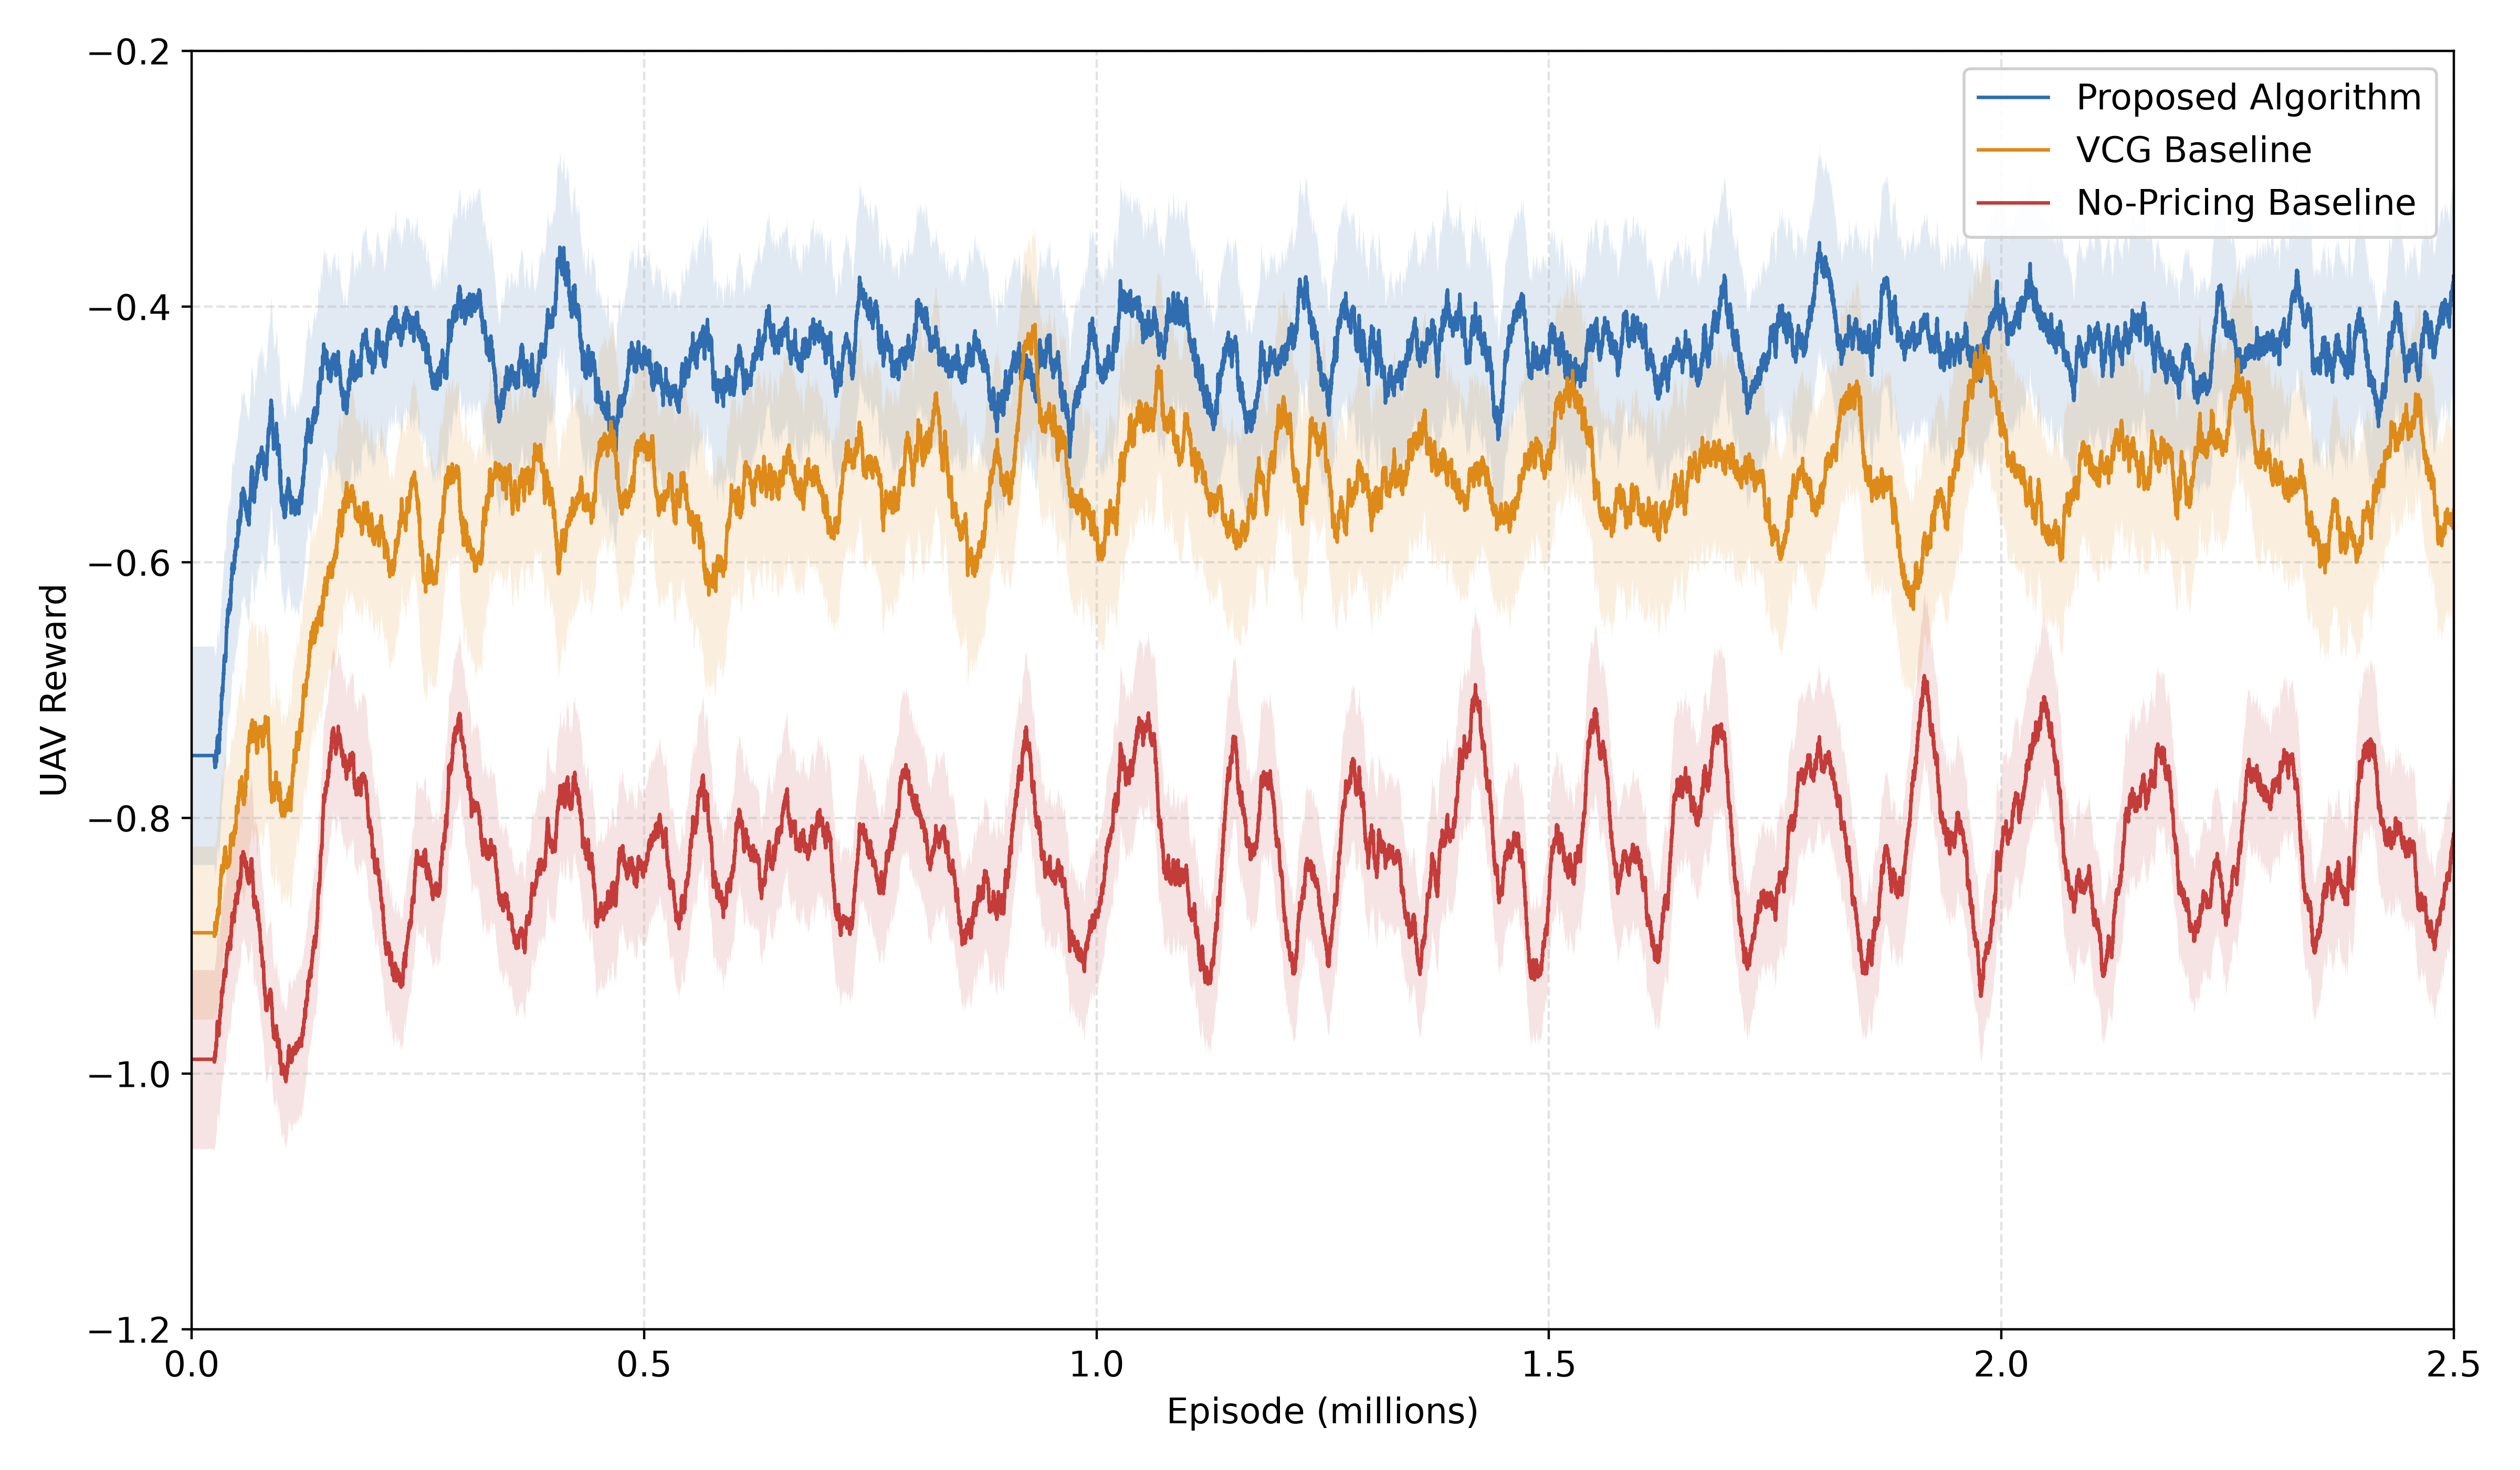
\includegraphics[width=\textwidth]{images/training_reward.png}
\caption{所提方法与两类基线的 UAV 训练回报。}
\label{fig:training-reward}
\end{figure}
图\ref{fig:training-reward}给出了三种方法的 UAV 训练回报演化。所提方法在初始探索阶段后迅速达到稳定区间，且在后续训练中始终保持最高的平均回报。相比之下，即时 VCG 定价基线虽能利用即时外部性改善资源分配，但其反事实价值评估较为局部，稳定回报仍低于所提方法；无定价基线的回报最低且波动更为显著。这表明，支付机制不仅影响用户的上报动机，也能通过反事实价值定价改善 UAV 对用户类型的识别与卸载决策。

\begin{figure}[H]
\centering
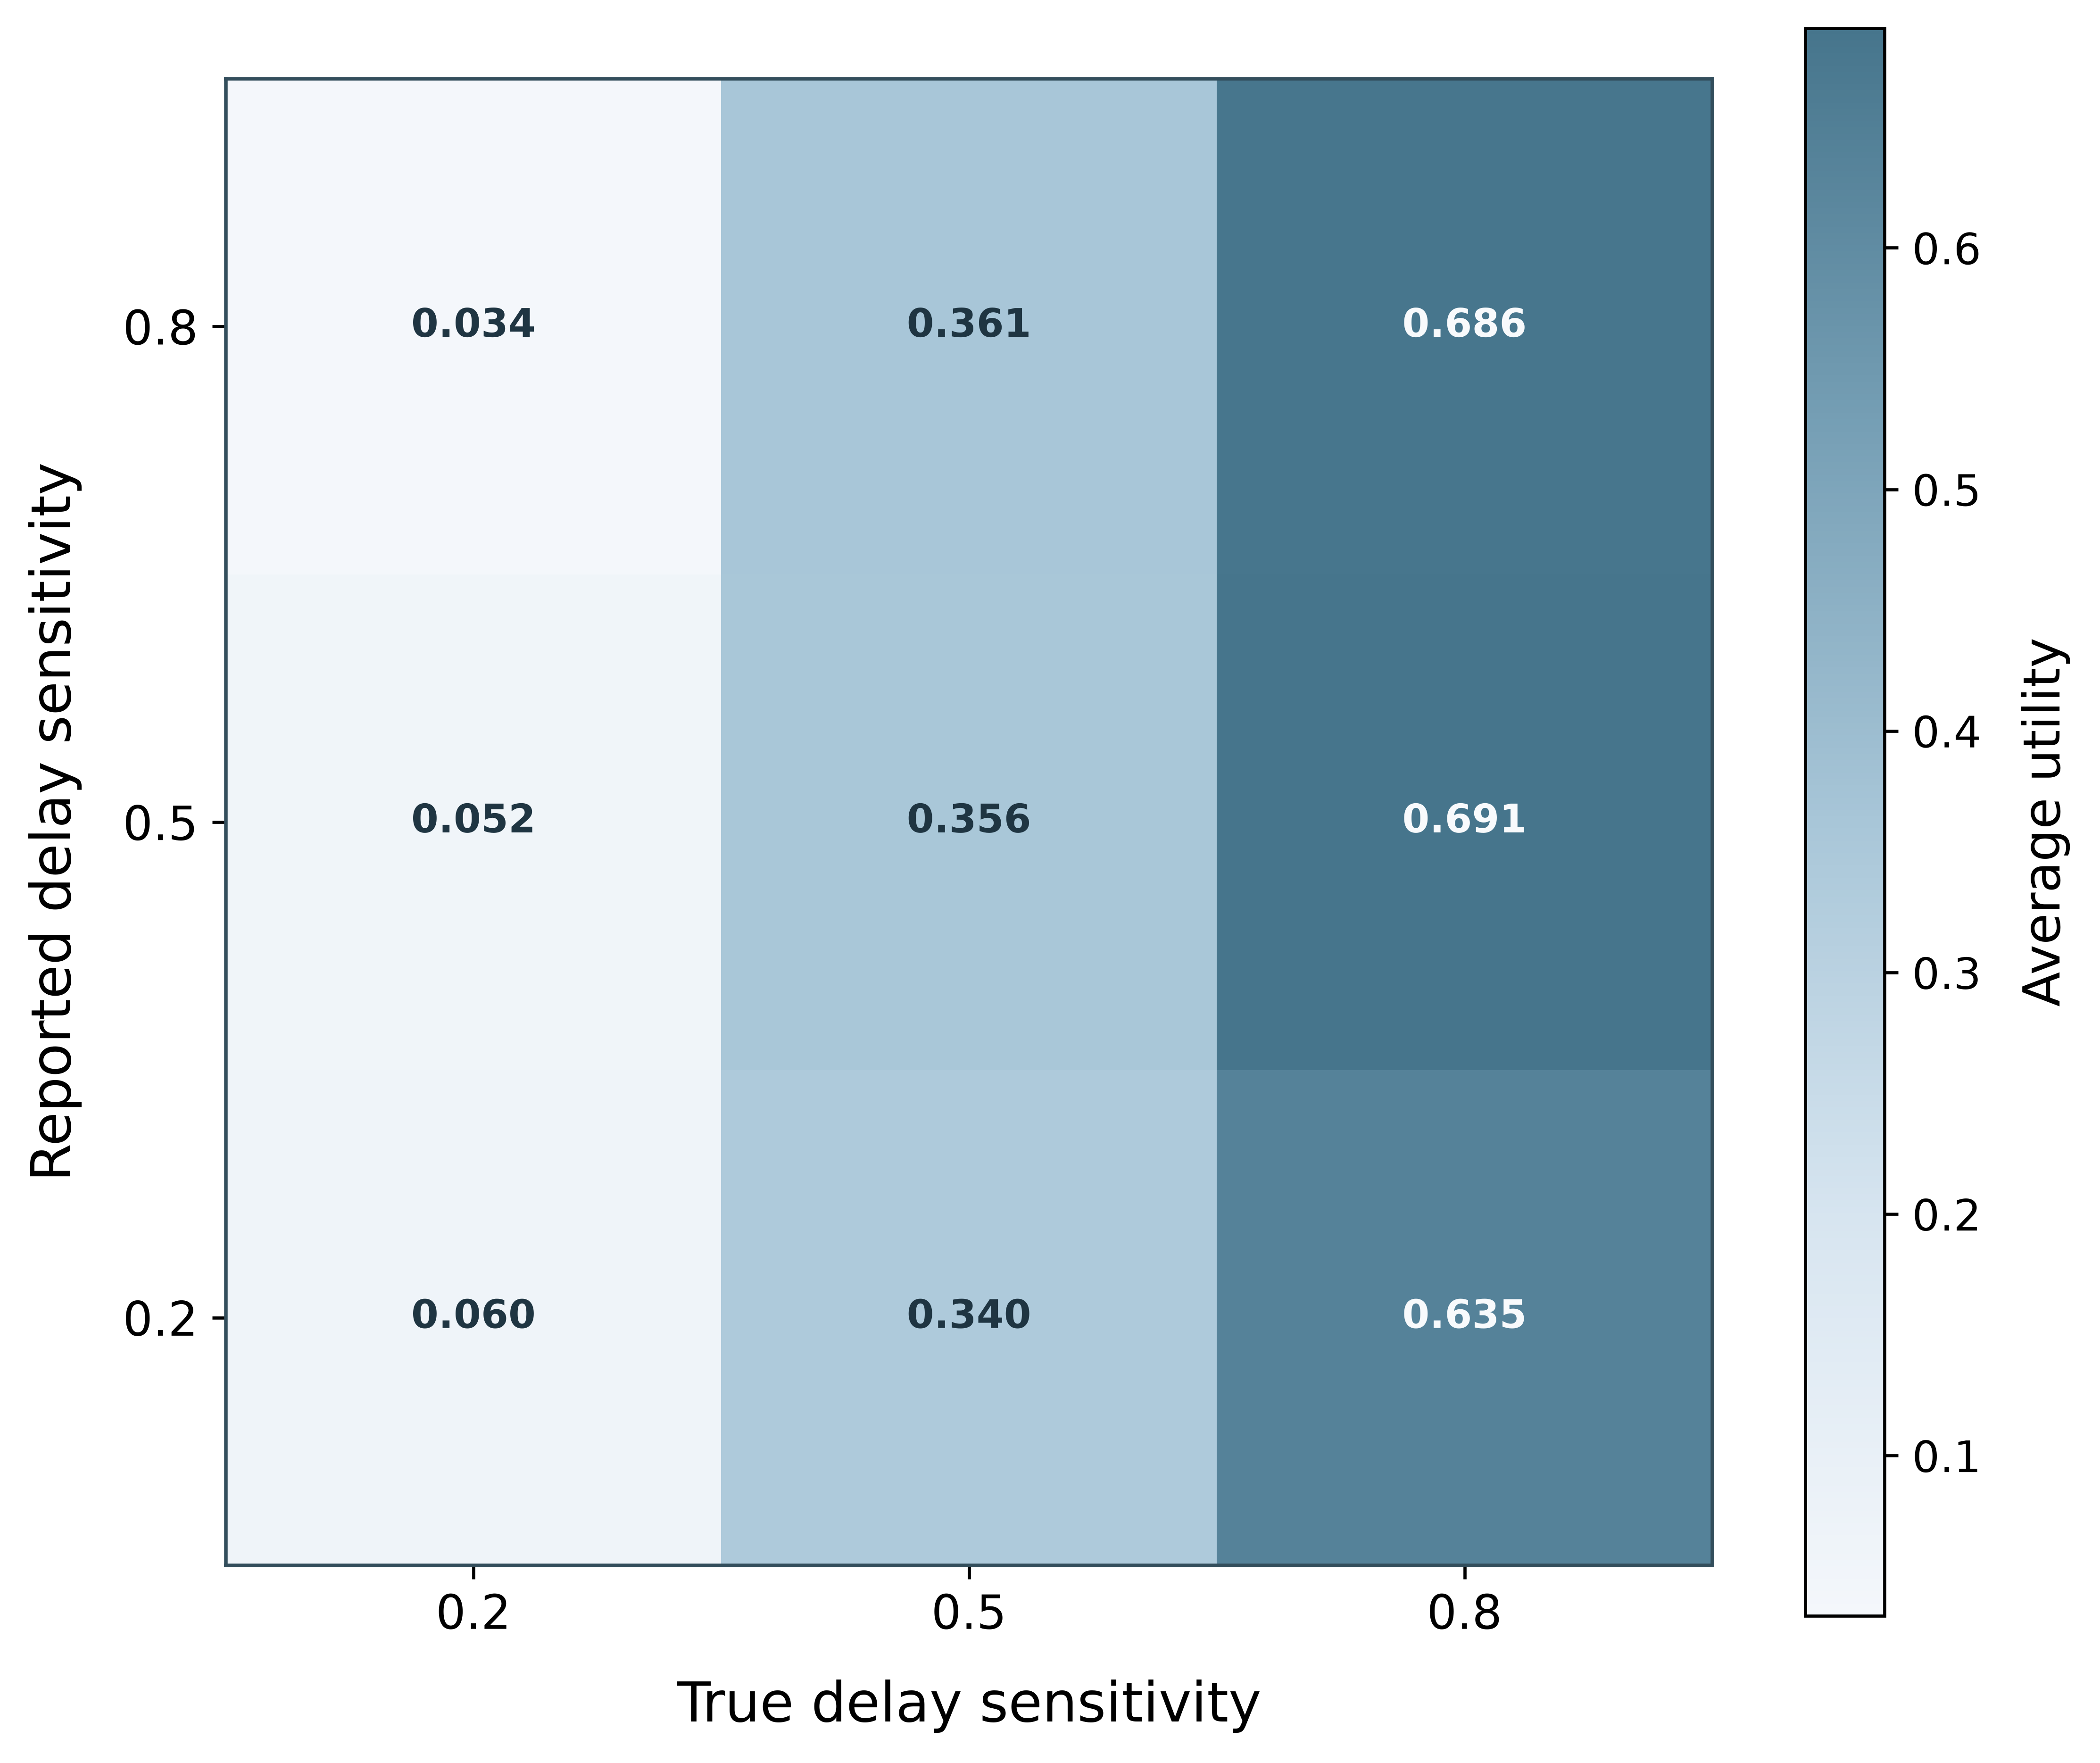
\includegraphics[width=0.78\textwidth]{images/utility_heatmap.png}
\caption{不同真实时延敏感系数和上报敏感系数下的平均用户效用。}
\label{fig:truth-misreport-utility}
\end{figure}

图\ref{fig:truth-misreport-utility}刻画了真实类型与上报类型对平均用户效用的共同影响。总体而言，用户效用随真实时延敏感系数提高而增大，表明资源分配能够优先服务于对时延更敏感的任务。对于低敏感用户（$\theta=0.2$），如实上报取得最高效用 $0.060$，而提高上报仅带来效用下降。对于中、高敏感用户，相邻上报水平之间的效用差异较小，最大偏离收益分别仅为 $0.005$ 和 $0.005$。因此，所提机制能够显著抑制虚报动机，并呈现近似激励相容性。

\begin{figure}[H]
\centering
\begin{subfigure}[b]{0.78\textwidth}
\centering
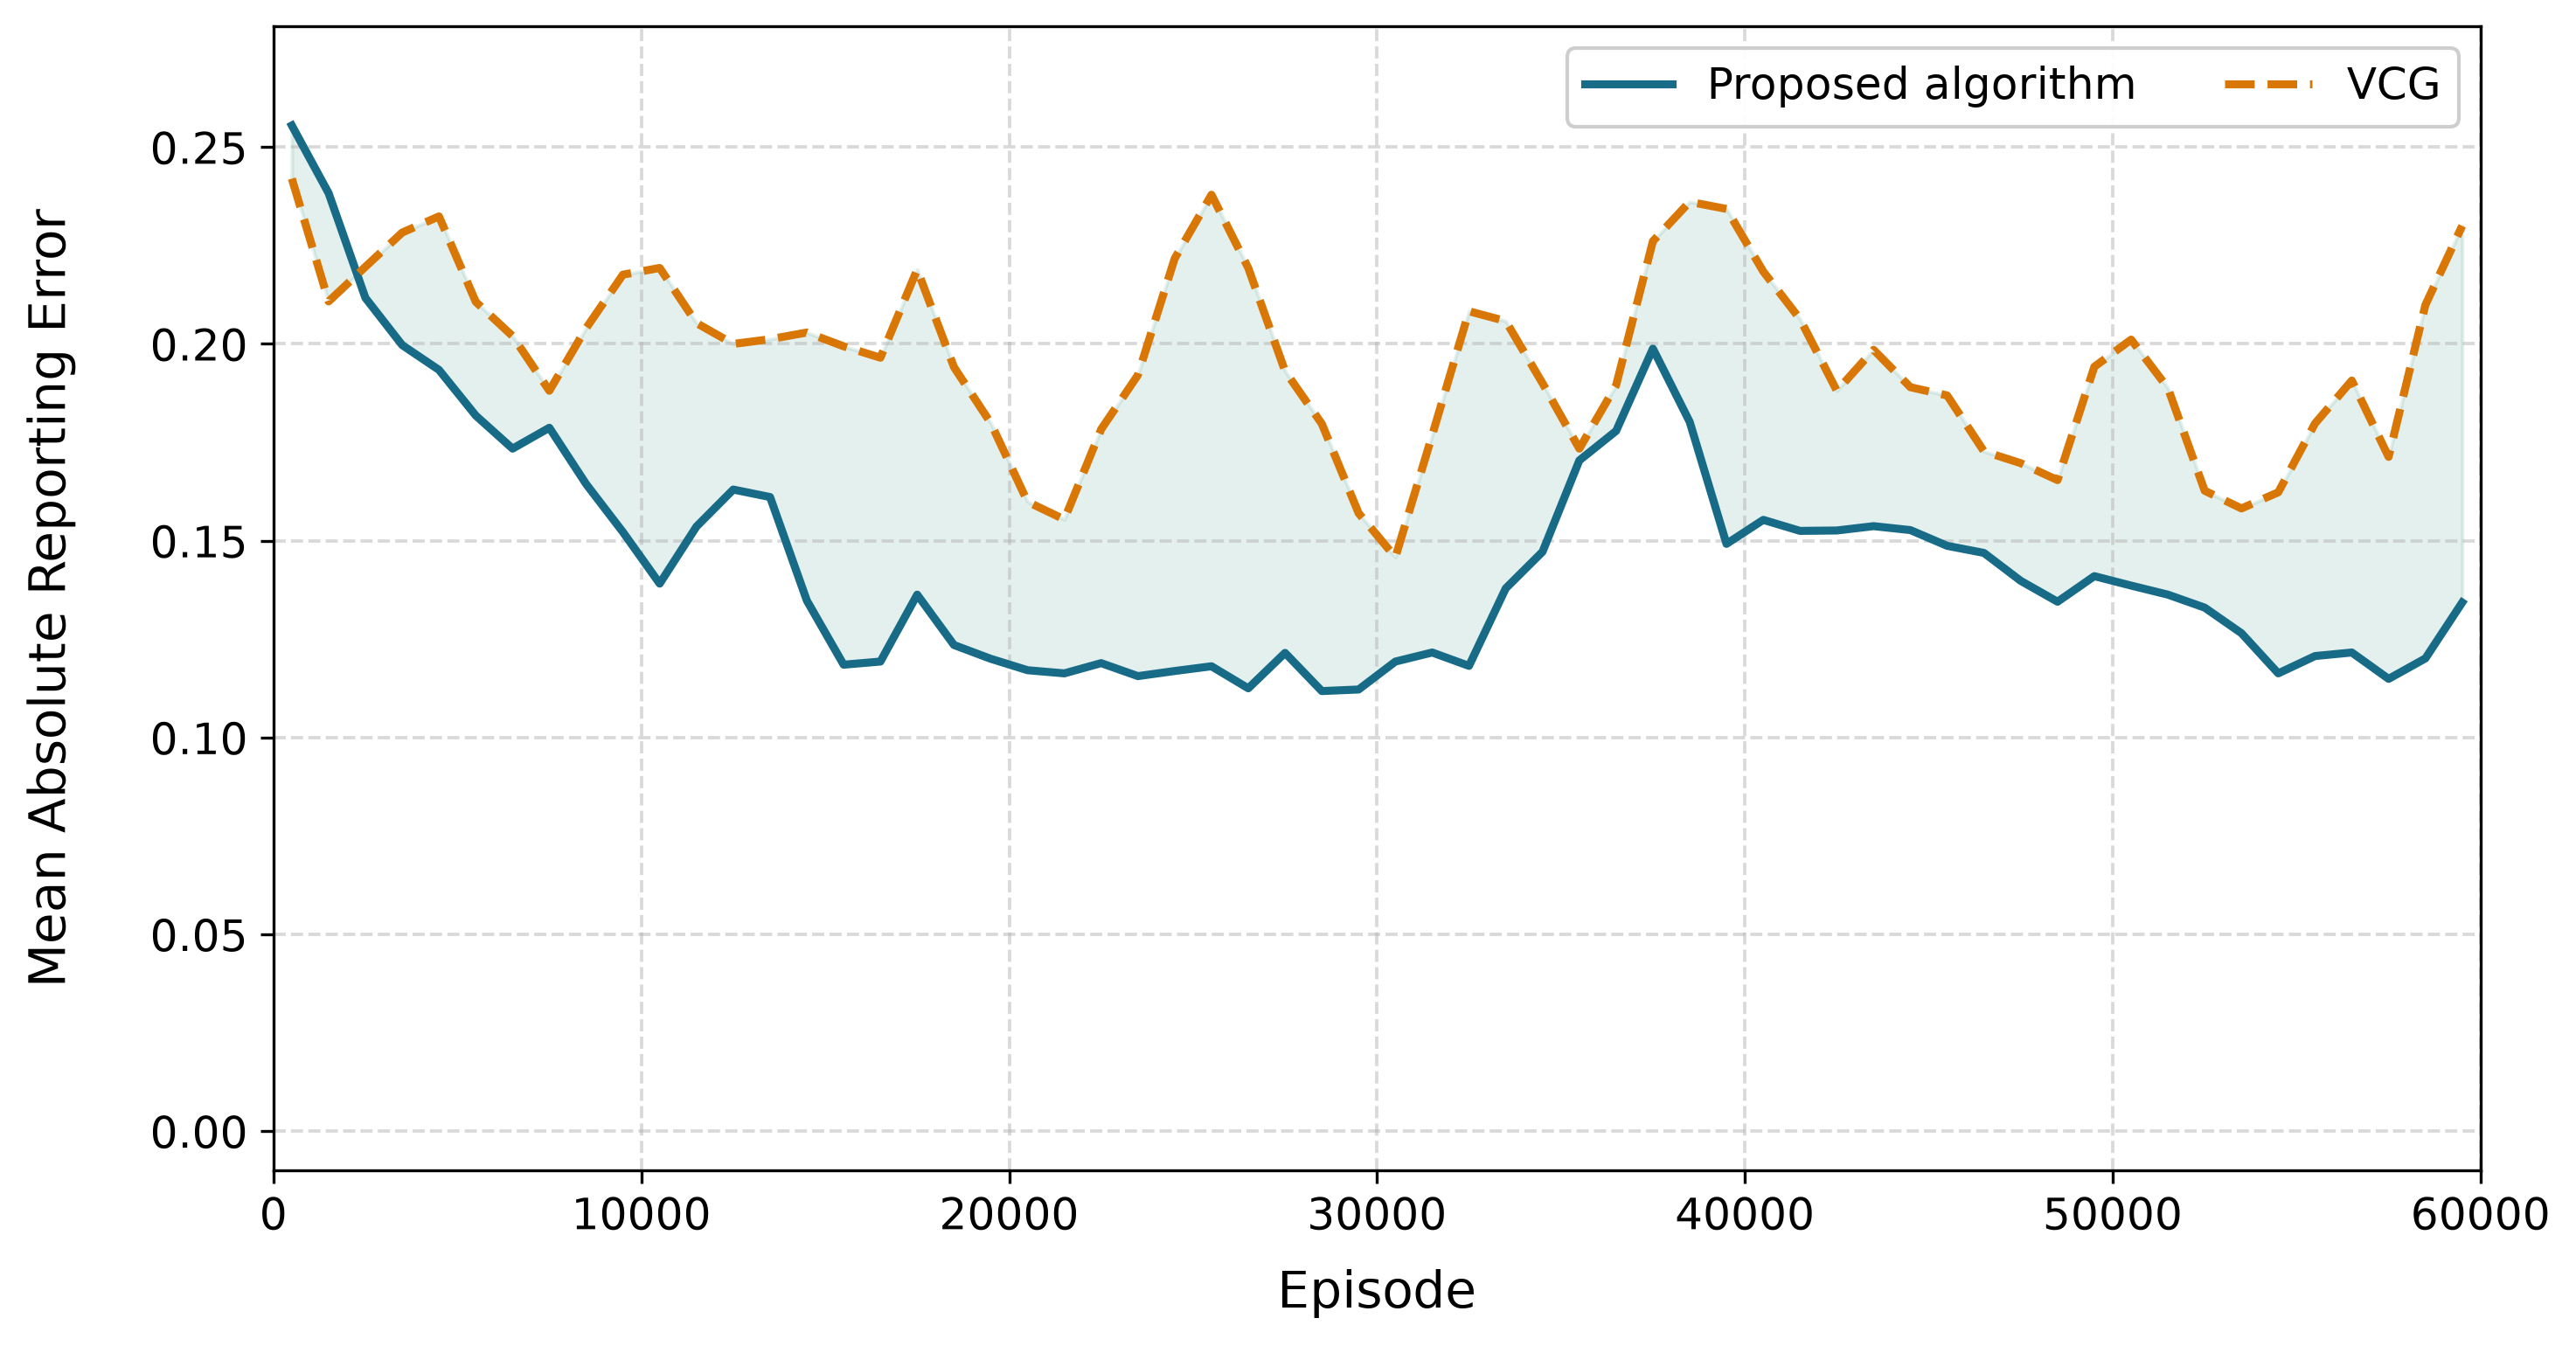
\includegraphics[width=\textwidth]{images/reporting_error_curve.png}
\caption{平均绝对上报误差的训练演化。}
\label{fig:reporting-error-curve}
\end{subfigure}

\vspace{0.5em}
\begin{subfigure}[b]{0.78\textwidth}
\centering
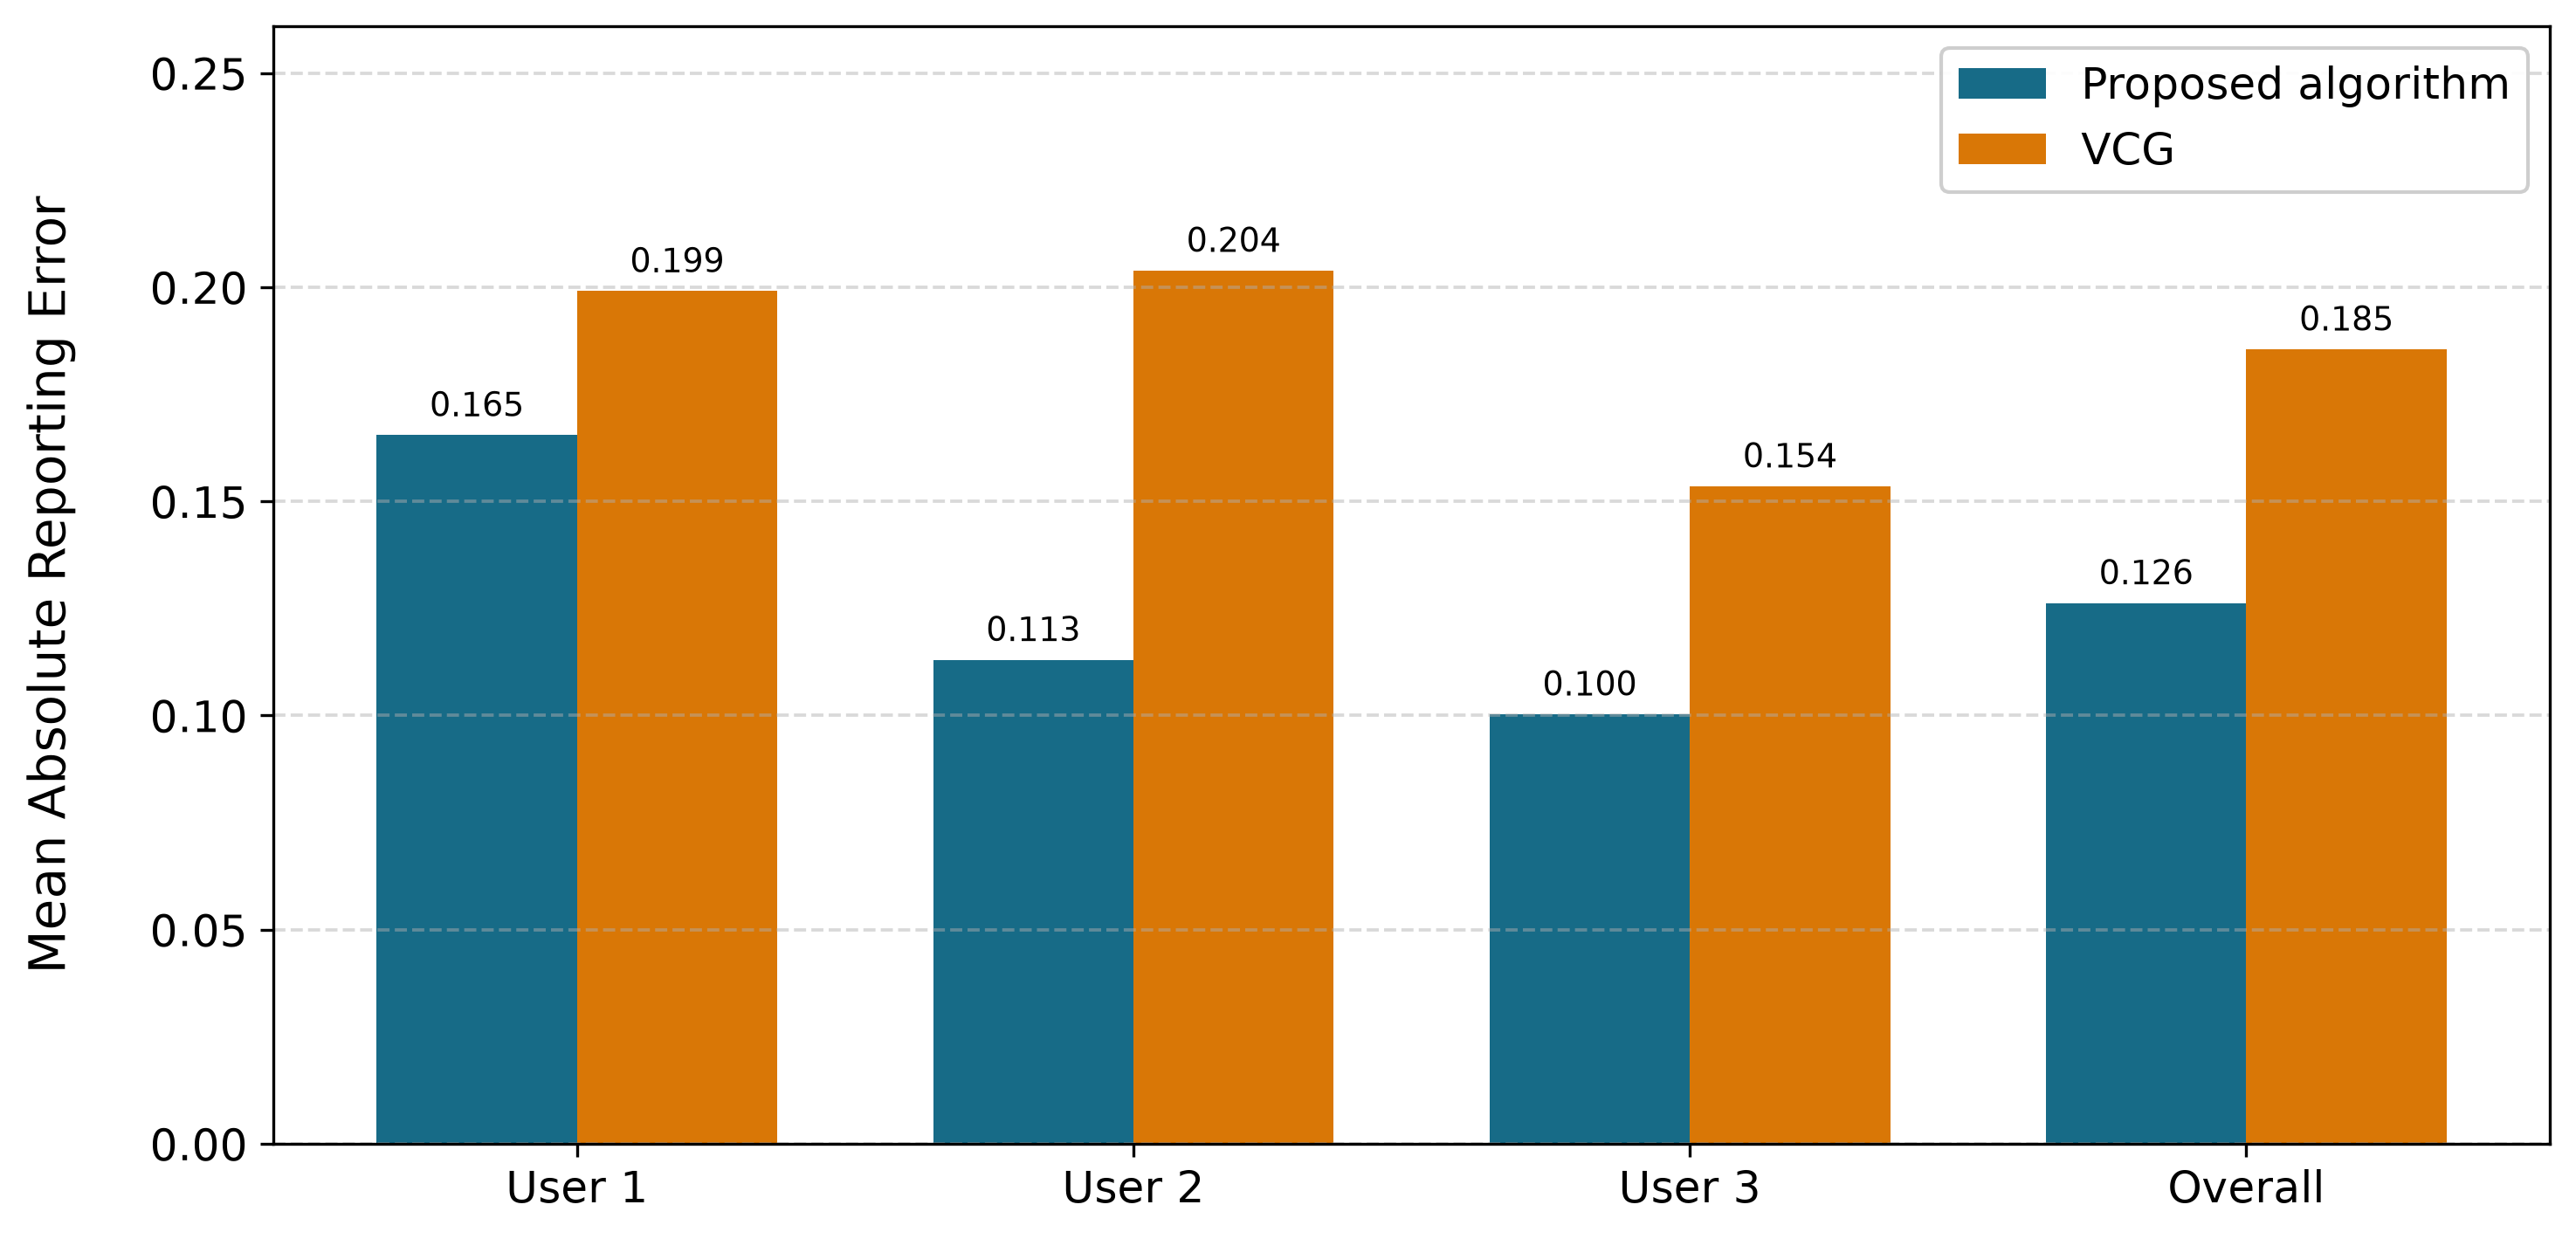
\includegraphics[width=\textwidth]{images/reporting_error.png}
\caption{各用户及总体平均绝对上报误差。}
\label{fig:reporting-error-bar}
\end{subfigure}
\caption{所提方法与即时 VCG 定价基线下的用户上报偏差。}
\label{fig:reporting-error}
\end{figure}

图\ref{fig:reporting-error}(a) 给出了平均绝对上报误差随训练过程的变化。经过初始探索后，所提方法的误差稳定在较低区间，且整体低于即时 VCG 定价基线，表明反事实价值定价能够持续抑制策略性虚报。图\ref{fig:reporting-error}(b) 进一步给出分用户比较：所提方法在三个用户上的平均绝对上报误差分别为 $0.165$、$0.113$ 和 $0.100$，均低于即时 VCG 定价基线对应的 $0.199$、$0.204$ 和 $0.154$。从总体指标看，所提方法将平均绝对上报误差由 $0.185$ 降至 $0.126$，说明其能够更有效地将用户收益与真实类型对齐。
\clearpage
\bibliographystyle{unsrt}
\bibliography{main}
\end{document}
